\documentclass{article}
\usepackage{amsmath}
\usepackage{braket}
\usepackage{amssymb}
\usepackage{hyperref}
\usepackage{booktabs}
\usepackage{graphicx}
\newcommand{\bfit}[1]{\textit{\textbf{#1}}}
\begin{document}
\textbf{\Large Chapter 8\\ Spin Qubit-Larmor Precession-Phase Shift Gate}\\\\\\
\textbf{8.1 Introduction}\\\\
In this chapter, we use an electron spin qubit under a constant external magnetic
field as an example to show how a single-qubit gate, namely, the phase shift gate,
can be implemented by turning the external magnetic field on for a given time.
This is \textit{not} a practical approach because turning on and off a large DC magenetic
field is difficult and cannot be done very fast. However, the example is very instructive
because it clarifies many important concepts in spin qubits by using relatively simple
mathematics.In the process, we will also discuss the contruction of Hamiltonian,
how Larmor precession can be understood on the Bloch sphere, and how to find the time
required to implement a given phase shift gate.\\\\\\
\bfit{\large 8.1.1 Learning Outcomes}\\\\
Be able to construct the Hamiltonian of a spin qubit under an external
magnetic field; understand the meaning of Larmor precession and its relationship
to a phase shift gate.\\\\
\bfit{8.1.2 Teaching Videos}\\\\
$\bullet$ Search for Ch8 in this playlist

- \url{https://tinyurl.com/3yhze3jn}\\\\
$\bullet$ Other videos

- \url{https://youtu.be/DtdDRfFb0Zs}\\\\\\
\textbf{\large 8.2 Construction of Single-Qubit Gate Hamiltonian Under a Constant Magnetic Field}\\\\
As discussed in Sect. 7.4, a charged particle with spin has its magnetic moment,
$\vec{\mu}$, interacts with an external magnetic field, $\vec{B}$, through the interaction
Hamiltonian in Eq. (7.10), which is repaeted here for convenience.
\begin{align*}\label{eq 8.1}
    H&=-\vec{B}\cdot\vec{\mu},\\
    &=-\vec{B}\cdot\gamma\vec{S}.\tag{8.1}
\end{align*}

In order to study how a general spin qubit evolves under this Hamiltonian,
we need to construct the Hamiltonian first. We will use \textit{electron spin}
as an example. Since an electron has a negative charge, $q=-e<0$, where $e=1.6\times10^{-19}C$,
its spin has an opposite direction to its spin magnetic moment, $\vec{\mu}$, with
$\gamma<0$ (Eq.(7.8) and Fig 7.4). Assuming the magentic field is constant and pointing at the 
\textit{negative} $\hat{z}$ direction (Fig.8.1 which is opposite to that in Fig.7.4), we have
$\vec{B}=-B_0\hat{z}$, where $B_0>0$. Therefore, a spin-up state, $\ket{\uparrow}$,
has a \textit{lower} energy than without the external magnetic field by
$|\vec{B}||\vec{\mu}|$ (Eq.(7.10)). This is the \textbf{ground state} and we can
label it as $\ket{g}$ or $\ket{0}$. Similarly, the spin-down state, $\ket{\downarrow}$, has a 
\textit{higher} energy than without the external magnetic field by $|\vec{B}||\vec{\mu}|$
and is an \textbf{excited state} ($\ket{e}$ or $\ket{1}$). Therefore,
\begin{align*}\label{eq 8.2}
    \ket{\uparrow}=\ket{g}=\ket{0},\\
    \ket{\downarrow}=\ket{e}=\ket{1}.\tag{8.2}
\end{align*}\\\\

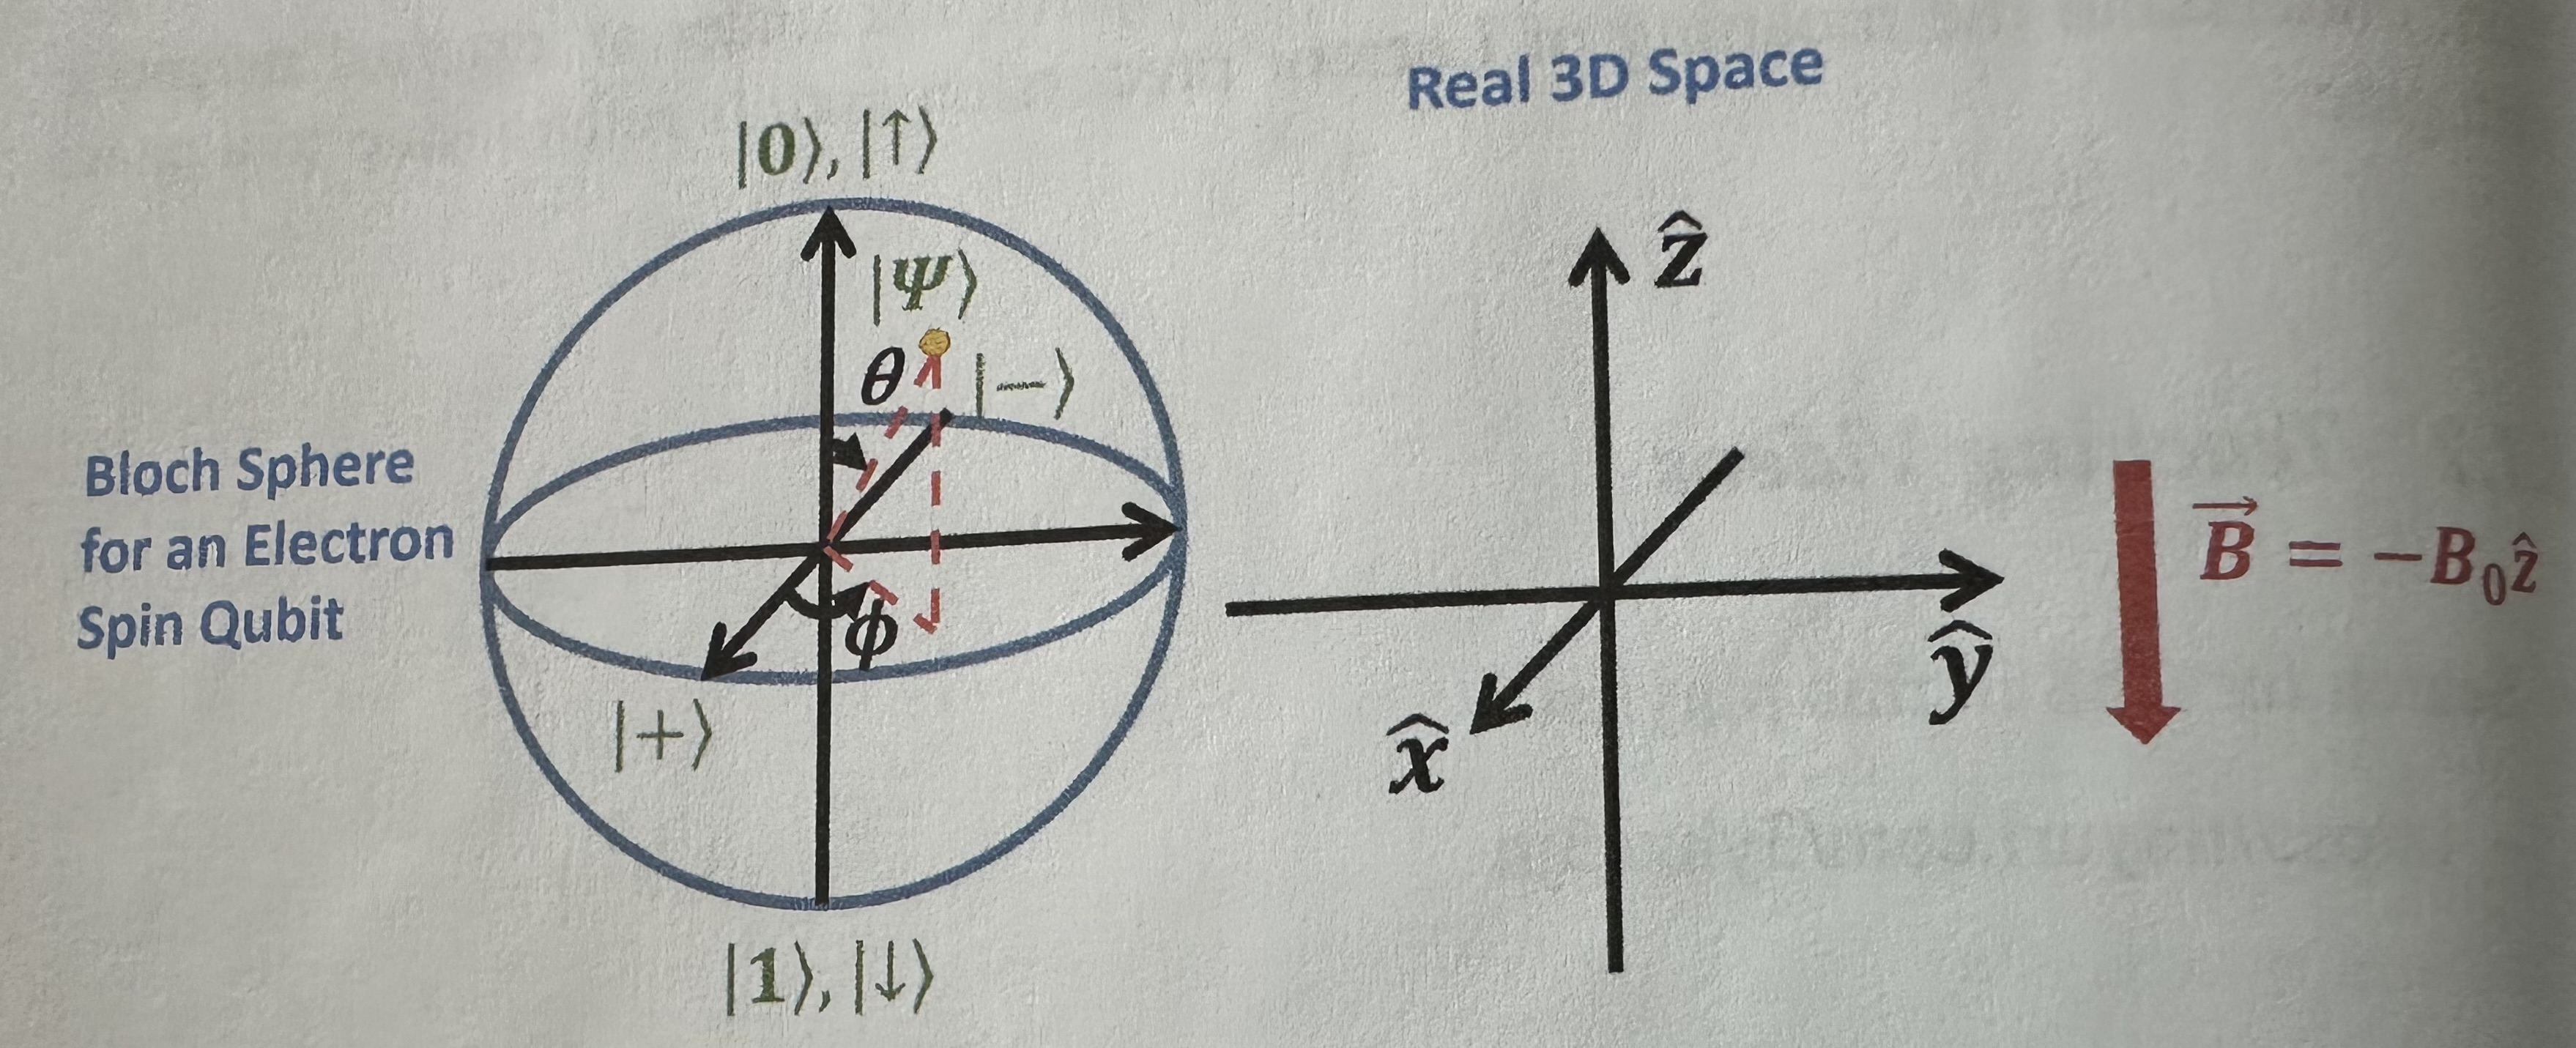
\includegraphics[scale=0.4]{Fig.8.1.jpeg}\\
\textbf{Fig. 8.1} The Bloch sphere representation of an electron spin
qubit and the real 3D space coordinate system in which the direction of the external
magetic field is shown\\

Before moving forward, \textit{there are a few confusions to be clarified}.
As discussed in Chap. 5 and 6 of this book and Chapter 27 of [1], the Bloch sphere
is the embedding of the abstract hyperspace in our real 3D space.
It has its uses but it also creates a few confusion. Firstly, the state on top of
the sphere does not have a higher energy although it appreas to be on the top.
Usually, it is labeled as $\ket{0}$ and is the ground state with the lowest
energy just like in this case. Therefore, do not think of it as a point on the top
of a ball which usually has a higher energy under gravitational force. Secondly, whether 
$\ket{0}$ or $\ket{1}$ has a higher energy depends on the charge of the particle
and the direction of the external magnetic field. In this chapter,
we assume the magnetic field is pointing downward so that the \textit{negatively}
charged electron spin has $\ket{0}$ as its ground state. It is completely legitimate 
if we point the magnetic field upward to have $\ket{1}$ as its ground state but it it
less commonly used. Similarly, if one wants to use a similiar convention for a positive charge
such as a hole, it will be more covenient to apply the magnetic field upward.

Now, we know how the enrgy splits or how the energy degeneracy it lifted under
an external magnetic field. We can construct the matrix for the Hamiltonian in Eq.
(\ref{eq 8.1}). If we conduct an experiment, we will observe two possible energy
values $\lambda_0=-|\vec{B}||\vec{\mu}|$ and $\lambda_1=|\vec{B}||\vec{\mu}|$, for a given
external magnetic field. We call them the eigenvalues of the obserbale operator (see also
 Sect. 3.4), which is just the Hamiltonian. In the experiment, we can also decide to call the corresponding eigenstates,
 $\ket{\uparrow}=\ket{0}$ and $\ket{\downarrow}=\ket{1}$, respectively. Using Eq. (3.9), we have,
 \begin{align*}\label{eq 8.3}
    H&=\sum_{i=0}^{1}\lambda_i\ket{i}\bra{i},\\
    &=-|\vec{B}||\vec{\mu}|\ket{\uparrow}\bar{\uparrow}+|\vec{B}||\vec{\mu}|\ket{\downarrow}\bar{\downarrow},\\
    &=-B_0|\vec{\mu}|\ket{0}\bra{0}+B_0|\vec{\mu}|\ket{1}\bra{1},\\
    &=-B_0|\vec{\mu}|\boldsymbol{\sigma_z}.\tag{8.3}
\end{align*}

The last step of Eq. (8.3) will be clear after the following derivation. From
Eqs. (7.7) and (7.9), for an electron, $|\vec{\mu}|=|g\frac{e}{2m}\hbar S|=\frac{-ge\hbar}{4m}\approx\frac{e\hbar}{2m}$,
which is just the \textbf{Bohr magneton} as expected. Note that $e>0$. Therefore,
\begin{align*}\label{eq 8.4}
    H&=B_0\frac{ge\hbar}{4m}\ket{0}\bra{0}-B_0\frac{ge\hbar}{4m}\ket{1}\bra{1},\\
    &=B_0\frac{ge\hbar}{4m}\begin{pmatrix}
        1\\0
    \end{pmatrix}
    \begin{pmatrix}
        1 \ 0
    \end{pmatrix}-B_0\frac{ge\hbar}{4m}
    \begin{pmatrix}
        0\\1
    \end{pmatrix}
    \begin{pmatrix}
        0 \ 1
    \end{pmatrix},\\
    &=B_0\frac{ge\hbar}{4m}\begin{pmatrix}
        1 \ 0\\ 0\ 0
    \end{pmatrix}-B_0\frac{ge\hbar}{4m}\begin{pmatrix}
        0\ 0\\ 0\ 1
    \end{pmatrix},\\
    &=B_0\frac{ge\hbar}{4m}\begin{pmatrix}
        1&0\\0&-1
    \end{pmatrix},\\
    &\approx -B_0\frac{e\hbar}{2m}\begin{pmatrix}
        1&0\\0&-1
    \end{pmatrix},\\
    &=-B_0\frac{e\hbar}{2m}\boldsymbol{\sigma_z},\tag{8.4}
\end{align*} 
where we have used the approximation that $g\approx-2$ from line 4 to line 5.
Note also that $-B_0\frac{e\hbar}{2m}<0$. It can be seen that the Hamiltonian
turns out to be proportional to the \textbf{Pauli spin matrix $\boldsymbol{\sigma_z}$}.
It can be better appreciated now why this is called the "spin" matrix and that the 
subscript z is due to the fact that the Hamiltonian is a result of a magenetic
field in the $\hat{z}$ direction (although it is pointing in $-\hat{z}$ in this case).\\\\
\textbf{\large 8.3 Larmor Precession and Phase Shift Gate}\\\\
Let us now apply the Schr\"{o}dinger equation to investigate how an electron spin qubit
state, $\ket{\Psi}$, will evolve under a constatn external magnetic field $\vec{B}=-B_0\hat{z}$.
Let $\ket{\Psi(t)}=\alpha(t)\ket{0}+\beta(t)\ket{1}$ to be arbitrary state at time $t$.
Based on Eqs. (4.1) and (\ref{eq 8.3}),
\begin{align*} \label{eq 8.5}
    i\hbar\frac{\partial \ket{\Psi}}{\partial t}&=H\ket{\psi},\\
    i\hbar\frac{\partial \ket{\Psi}}{\partial t}&=-B_0|\vec{\mu}|\boldsymbol{\sigma_z}\ket{\psi},\\
    i\hbar\frac{\partial}{\partial t}\begin{pmatrix}
        \alpha(t)\\ \beta(t)
    \end{pmatrix}&=-B_0|\vec{\mu}|\begin{pmatrix}
        1&0\\0&-1
    \end{pmatrix}
    \begin{pmatrix}
        \alpha(t)\\ \beta(t)
    \end{pmatrix},\\
    \begin{pmatrix}
        i\hbar\frac{\partial\alpha(t)}{\partial t}\\
        i\hbar\frac{\partial\beta(t)}{\partial t}
    \end{pmatrix}&=\begin{pmatrix}
        -B_0|\vec{\mu}\alpha(t)\\
        B_0|\vec{\mu}|\beta(t)
    \end{pmatrix}.\\ \tag{8.5}
\end{align*}

By equating the vector elements on the left and right sides of the equation, we obtain
two equations,
\begin{align*}
    \label{eq 8.6} i\hbar\frac{\partial\alpha(t)}{\partial t}&= -B)o|\vec{\mu}|\alpha (t), \tag{8.6}\\
    \label{eq 8.7} i\hbar\frac{\partial \beta(t)}{\partial t}&= B_0|\vec{\mu}|\beta(t).\tag{8.7}\\
\end{align*}

There are two first-order differential equations for $\alpha(t)$ and $\beta(t)$, respectively.
The solution are,
\begin{align*}
    \label{eq 8.8}\alpha(t)&=\alpha_0exp\left\{\frac{-B_0|\vec{\mu}|}{i\hbar}t\right\},\tag{8.8}\\
    \label{eq 8.9}\beta(t)&=\beta_0exp\left\{\frac{B_0|\vec{\mu}|}{i\hbar}t\right\}. \tag{8.9}
\end{align*}
where $\alpha_0$ and $\beta_0$ are two complex number constants. When $t=0, \alpha(t)=\alpha_0$ and $\beta(t)=\beta_0$.
This just represents the initial state before the magnetic field is applied. One may verify the solutions
by substituting them into Eqs. (\ref{eq 8.6}) and (\ref{eq 8.7}).
Apparently, the coefficients of $\ket{\Psi}$ are changing as a function of time due to the interaction
Hamiltonian between the spin magnetic moment and the external magnetic field. Therefore,
$\ket{\Psi(t)}$ moves on the Bloch sphere when the magnetic field is applied.

To understand how it moves, let us represent $\ket{\Psi}$ in the polar ($\theta$) and
azimuthal ($\phi$) angles on the Bloch sphere (Eq. (5.3)). We first set $\alpha_0=\cos{\frac{\theta_0}{2}exp\left\{-i\frac{\phi_0}{2}\right\}}$
and $\beta_0=\sin{\frac{\theta_0}{2}exp\left\{i\frac{\phi_0}{2}\right\}}$, where $\theta_0$ and
$\phi_0$ are the initial angles of the state on the Bloch sphere. Then from Eqs. (\ref{eq 8.8}) and
(\ref{eq 8.9}),
\begin{align*} \label{eq 8.10}
    \Ket{\Psi(t)}=&\alpha(t)\ket{0}+\beta(t)\ket{1},\\
    =&\alpha_0exp\left\{\frac{-B_0|\vec{\mu}|}{i\hbar}t\right\}\ket{0}+
    \beta_0exp\left\{\frac{B_0|\vec{\mu}|}{i\hbar}t\right\}\ket{1},\\
    =&\cos{\frac{\theta_0}{2}}exp\left\{-i\frac{\phi_0}{2}\right\}exp\left\{\frac{-B_0|\vec{\mu}|}{i\hbar}t\right\}\ket{0}\\
    &+\sin{\frac{\theta_0}{2}exp\left\{i\frac{\phi_0}{2}\right\}}exp\left\{\frac{B_0|\vec{\mu}|}{i\hbar}t\right\}\ket{1},\\
    =&\cos{\frac{\theta_0}{2}}exp\left\{-i\frac{\phi_0-2B_0|\vec{\mu}|t/\hbar}{2}\right\}\ket{0}\\
    &+\sin{\frac{\theta_0}{2}}exp\left\{i\frac{\phi_0-2B_0|\vec{\mu}|t/\hbar}{2}\right\}\ket{1},\\
    =&\cos{\frac{\theta_0}{2}}exp\left\{-i\frac{\phi}{2}\right\}\ket{0}+\sin{\frac{\theta_0}{2}}exp\left\{i\frac{\phi}{2}\right\}\ket{1},\tag{8.10}
\end{align*}
where we finally mad the substitution of $\phi=\phi_0-2B_0|\vec{\mu}|t/\hbar$. The polar angle does not
change and stays onstant at $\theta_0$ but the azimuthal angle changes at a rate of 
$\frac{\partial\phi}{\partial t}= -2B_0|\vec{\mu}|/\hbar$ which means the qubit state will rotate
clockwise (looking from the top) as shown in the left part of Fig. 8.2 (the right part will be explained in the nex sub-section).
This is called the \textbf{Larmor precession} and the precession rate is called the 
\textbf{Larmor frequency}, $\omega_L=2B_0|\vec{\mu}|/\hbar$ (this is an angular frequency and\\

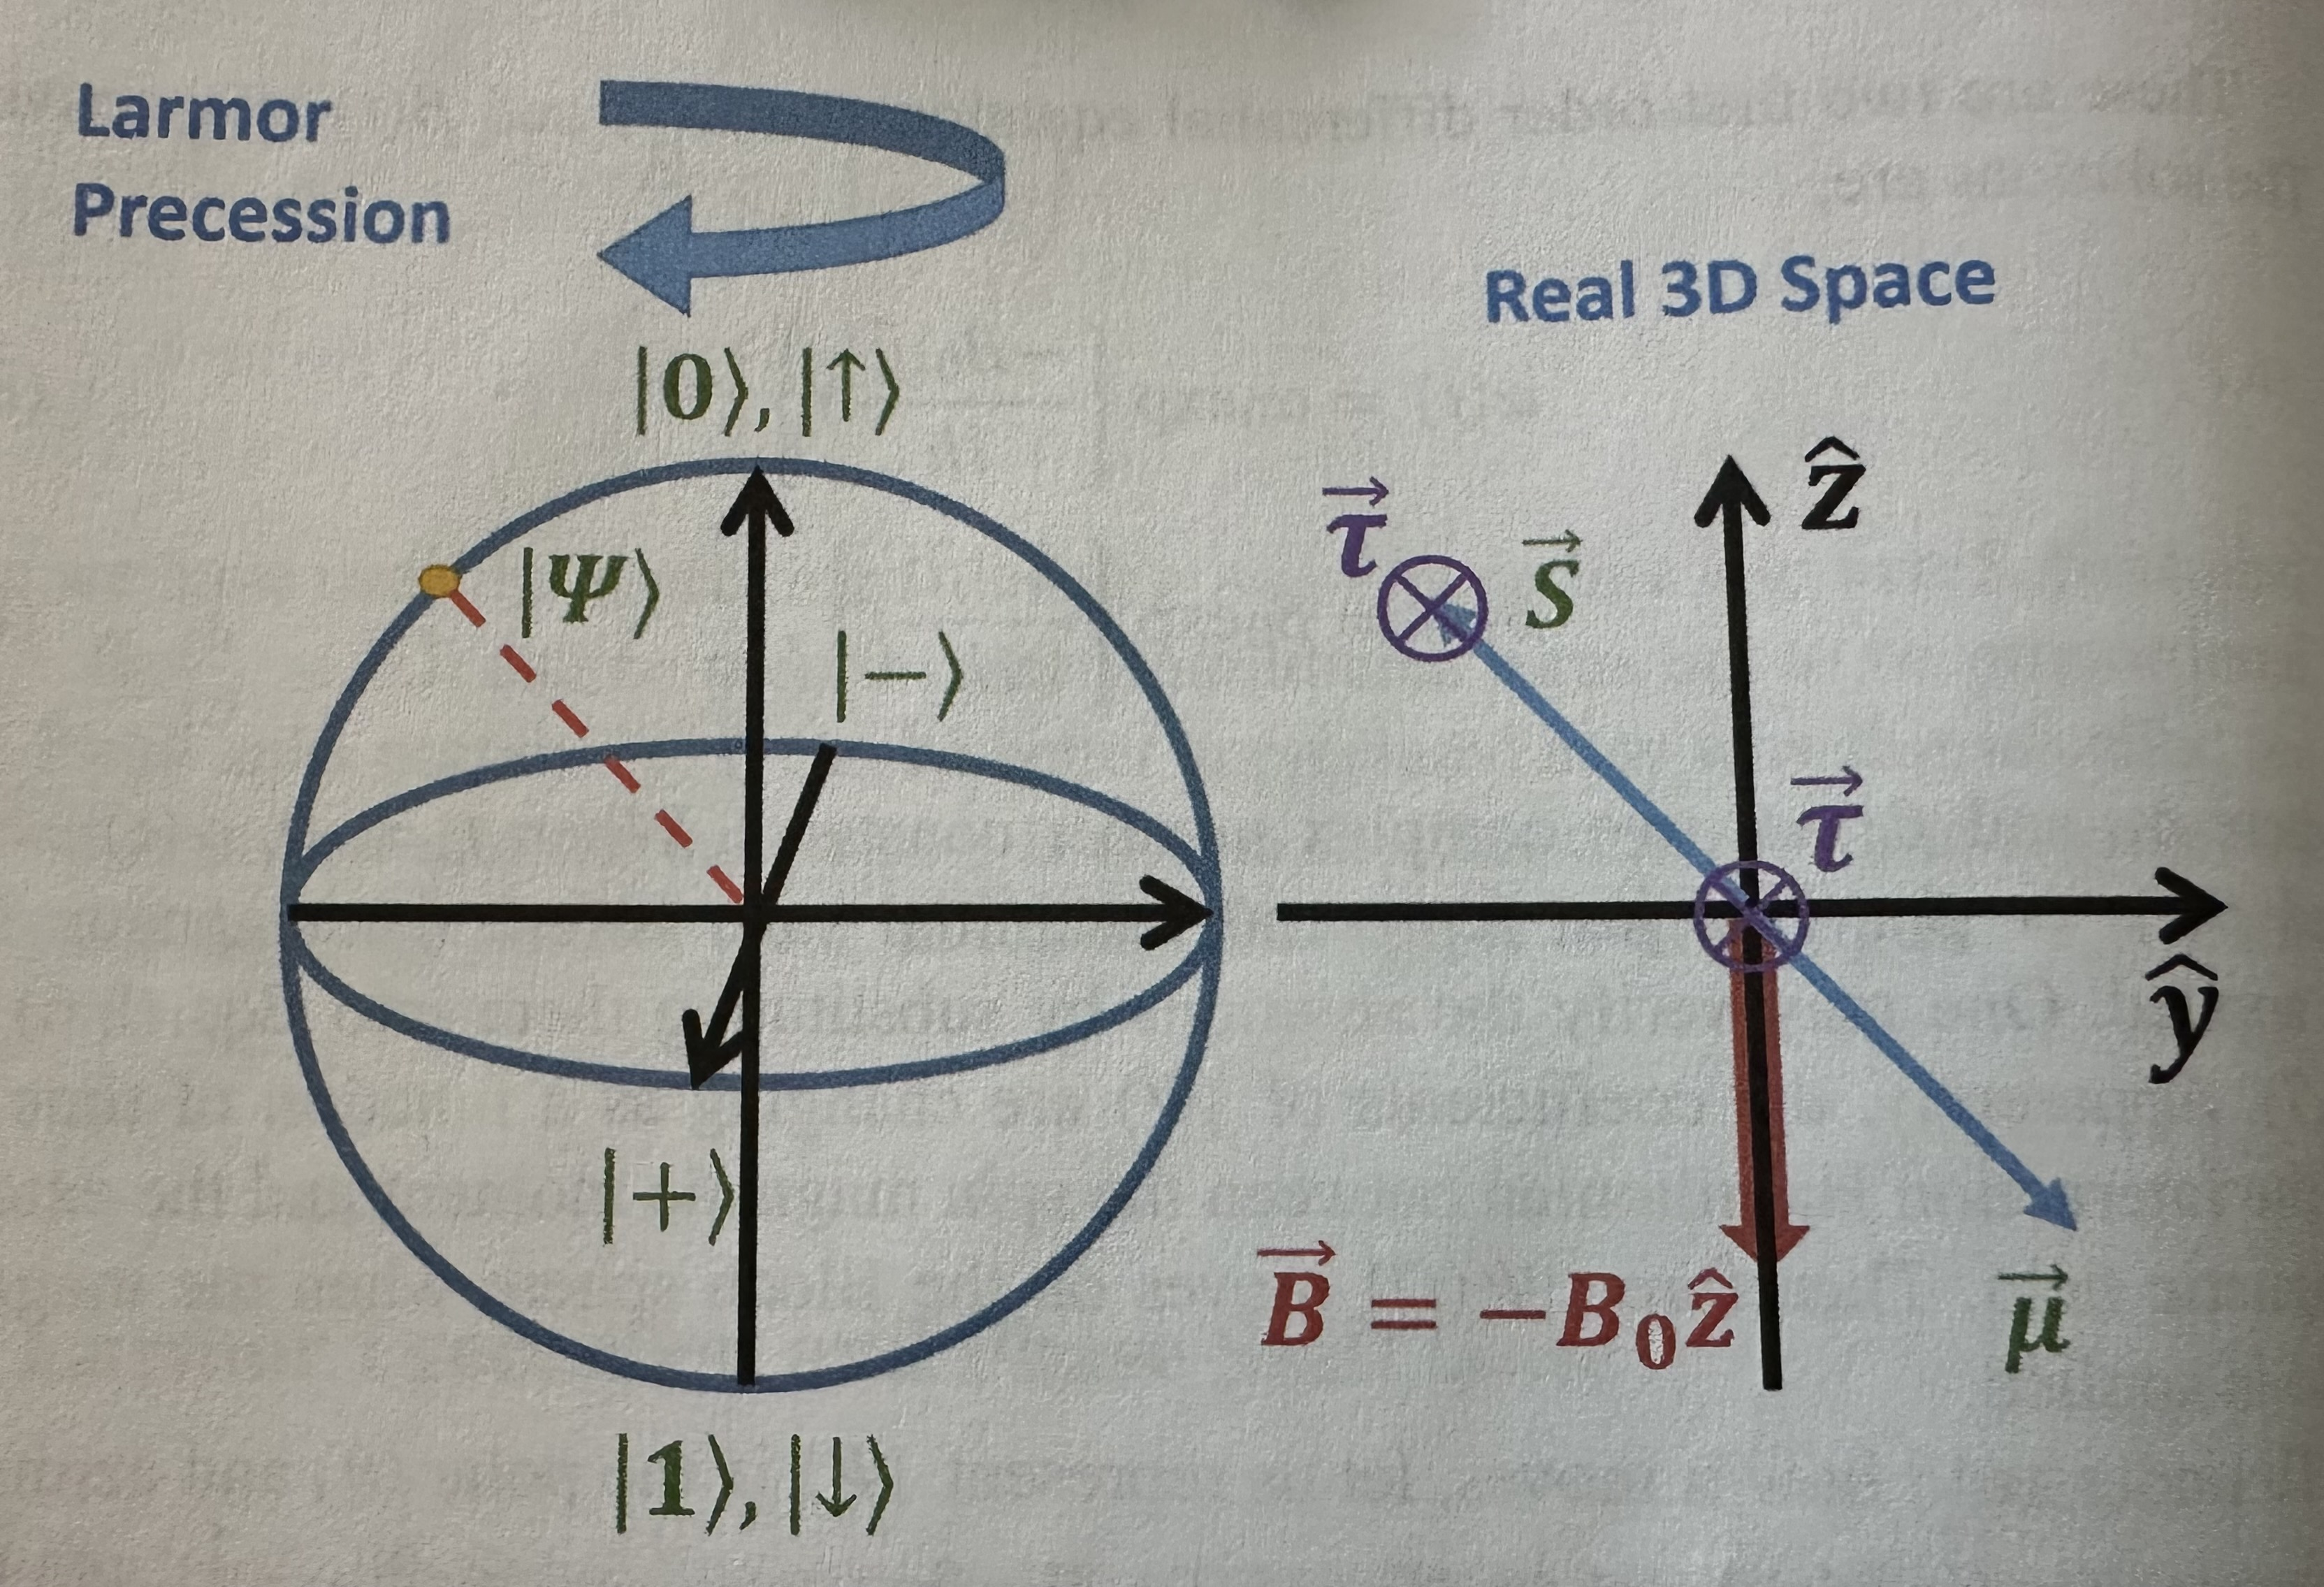
\includegraphics[scale=0.35]{Fig.8.2.jpeg}\\
\textbf{Fig. 8.2} The Bloch sphere representation of an electron spin qubit and the corresponding spin
angular momentum, $\vec{S}$, and spin magnetic moment, $\vec{\mu}$, in the real 3D space. The torque, $\vec{\tau}$,
generated by the interaction between $\vec{B}$ and $\vec{\mu}$ is also shown at the original.
\\\\
we also taken its absolute value since the precession direction is immaterial
in the definition). It can also be further expressed as 
\begin{align*}\label{eq 8.11}
    \omega_L&=2B_0|\vec{\mu}|/\hbar,\\
    &=2B_0|\gamma\vec{S}|/\hbar,\\
    &=\left|\frac{2ge\hbar}{4m}B_0\right|/\hbar,\\
    &\approx\frac{e}{m}B_0.\tag{8.11}
\end{align*}
We can also define
\begin{equation} \label{eq 8.12}
    f_L=\frac{\omega_L}{2\pi}. \tag{8.12}
\end{equation}

From the first line of Eq. (\ref{eq 8.11}), we can rewrite the eigenenergies of the system
(Sect. 8.2) as
\begin{align*}\label{eq 8.13}
    \lambda_0&=-|\vec{B}||\vec{\mu}|,\\
    &=-\hbar\omega_L/2.\tag{8.13}
\end{align*}

and
\begin{align*}\label{eq 8.14}
    \lambda_1&=|\vec{B}||\vec{\mu}|,
    &=\hbar\omega_L/2.\tag{8.14}
\end{align*}

Therefore, the separation of the two energy levels ($\lambda_1-\lambda_0$) 
determines the Larmor frequency.\\\\\\
\bfit{\large 8.3.1 Notes on Qubit Larmor Precession}\\\\
\textit{This subsection may be skipped if you are not interesed in going deeper}.
It is instructive to look deeper into the physics of Larmor precession and its relationship 
with the qubit on the Bloch sphere. The physics behind Larmor precession is due to the \textbf{torque},
$\vec{\tau}$, which is generated by the interaction between the magnetic field,
$\vec{B}$, and the spin magnetic moment,$\vec{\mu}$, \textit{changing the spin angular momentum}, $S$.
The torque is found by,
\begin{equation}\label{eq 8.15}
    \vec{\tau}=\vec{\mu}\times\vec{B}. \tag{8.15}
\end{equation}

Figure 8.2 shows that for a state $\ket{\Psi}$ on the Bloch sphere embedding in the real
3D space, it has a corresponding spin angular momentum $\vec{S}$ on the y-z plane. Since an electron
has a negative charge, the corresponding magnetic moment, $\vec{\mu}$, is in the opposite direction
but along the same line. Using the right-hand rule, a torque $\tau$ is generated deu to Eq. (\ref{eq 8.5})
which is pointing into the screen/paper. Note that his torque will modify 
$\vec{S}$ but not $\vec{\mu}$ because the torque is \textit{the rate of change of angular momentum}
(although the spin magnetic moment is the cause of the torque) through the following equation:
\begin{equation}\label{eq 8.16}
    \vec{\tau}=\frac{\partial \vec{S}}{\partial t}. \tag{8.16}
\end{equation}

Therefore, the aungular momentum moves away from the $y-z$ plane into
the paper. In the Bloch sphere, this corresponds to the state $\ket{\Psi}$
precessing clockwise when looking from the top.\\\\\\
\textbf{\large 8.4 Inplementation of Phase Shift Gate}\\\\
A phase shift gate, $\boldsymbol{U_{PS,\varPhi}}$, with a phase $\Phi$ has the following
matrix (Eq.(4.41)):
\begin{equation}\label{eq 8.17}
    \boldsymbol{U_{PS,]Phi}}=\begin{pmatrix}
        1&0\\0&e^{i\phi}
    \end{pmatrix}\tag{8.17}
\end{equation}

How to implement a general phase shift gate using the physics setup we have (i.e., an electron spin
qubit under a constant external magnetic field)? Based on the discussion in the previous section,
the qubit will rotate about the vertical axis on the Bloch sphere at Larmor frequency
\textit{clockwise} when the external magnetic field is turned on. What is the meaning of a phase
shift gate? It is a \textit{counterclockwise} rotation about the vertical axis by an angle
$\Phi$. This can be understood through Eq.(5.4) with $\lambda=0,\theta=0,\alpha=0,$ and $\phi=0$ as the
third counterclockwise rotation (Fig. 5.2). Therefore, they have the same action except in the opposite
direction. Figure 8.3. shows that the phase shift gate, $\boldsymbol{U_{PS,\varPhi}}$, rotates the state
by an angle $\varPhi$ \textit{anti-clockwise} when looking from the top. Therefore, we need to use
our setup to achieve the same effect by rotating it clockwise by $2\pi-\varPhi$.
As a specific example, a $\boldsymbol{U_{PS,\pi}}$ is just \bfit{Z}-gate (or $\boldsymbol{\sigma_z}$) and
it can be achieved by rotating the state about the vertical axis clockwise by $\pi$ (Fig. 8.3).

Now let us look at the equation and find out how much time we need to turn on
the external magnetic field to achieve a desirable rotation. From the second line of
Eq. (\ref{eq 8.10})\\

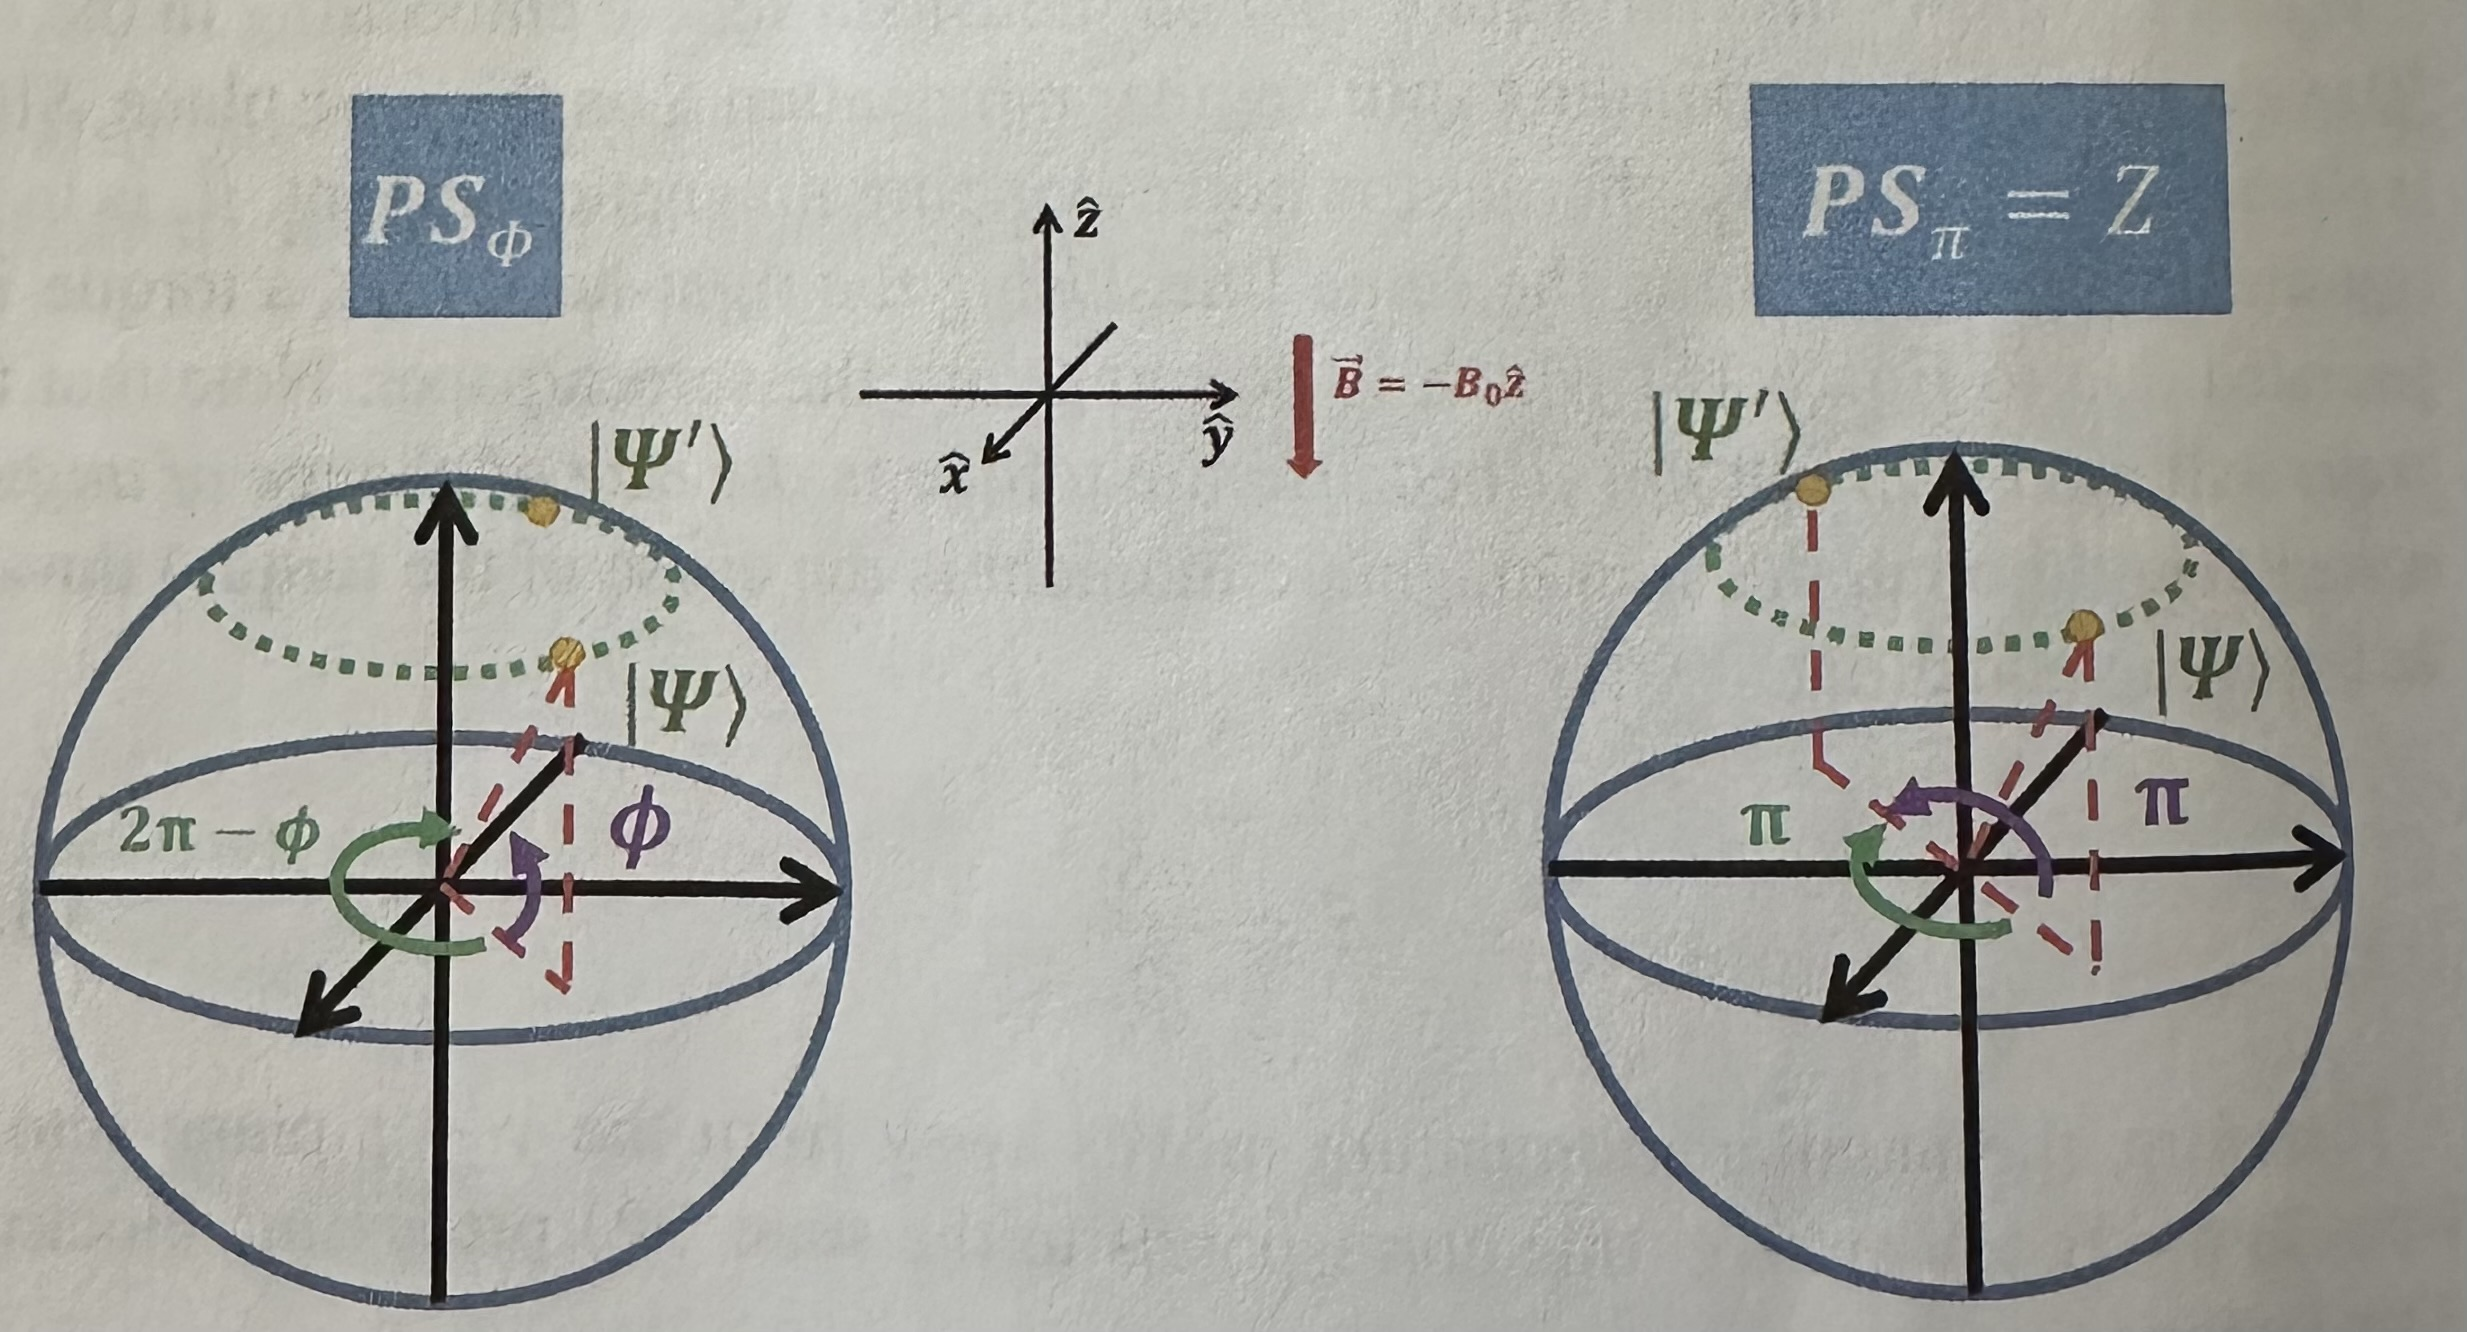
\includegraphics[scale=0.5]{Fig.8.3.jpeg}\\
\textbf{Fig.8.3} Illustration of the action of phase shife gate. $\boldsymbol{U_{PS,\varPhi}}$, on a general qubit
on the Bloch sphere (left: general, right: Z-gate). It can be implemented using an electron qubit under a vertical 
external magnetic field by rotating $2\pi-\varPhi$\\\\
\begin{align*}\label{eq 8.18}
    \ket{\varPsi(t)}&= \alpha(t)\ket{0}+\beta(t)\ket{1}=\begin{pmatrix}
        \alpha(t)\\ \beta(t)
    \end{pmatrix},\\
    &=\alpha_0\exp\left\{\frac{-B_0|\vec{\mu}|}{i\hbar}t\right\}\ket{0}+\beta_0\exp\left\{\frac{B_0|\vec{\mu}|}{i\hbar}t\right\}\ket{1},\\
    &=\begin{pmatrix}
        \exp\left\{\frac{-B_0|\vec{\mu}|}{i\hbar}t\right\}&0\\
        0&\exp\left\{\frac{B_0|\vec{\mu}|}{i\hbar}t\right\}
    \end{pmatrix}\begin{pmatrix}
        \alpha_0\\ \beta_0
    \end{pmatrix},\\
    &=\begin{pmatrix}
        \exp\left\{i\frac{e}{2m}B_0t\right\}&0\\
        0&\exp\left\{-i\frac{e}{2m}B_0t\right\}
    \end{pmatrix}\begin{pmatrix}
        \alpha_0\\ \beta_0
    \end{pmatrix},\\
    &=\exp\left\{i\frac{e}{2m}B_0t\right\}\begin{pmatrix}
        1&0\\0&\exp\left\{-i\frac{e}{m}B_0t\right\}
    \end{pmatrix}\begin{pmatrix}
        \alpha_0\\ \beta_0
    \end{pmatrix}.\tag{8.18}
\end{align*}\\
In line 1, we write the state in both the $bra-ket$ notation and column vector form.
Line 3 shows that the state at any times is equal to matrix multiplying the initial
state, $\begin{pmatrix}
\alpha_0\\ \beta_0    
\end{pmatrix}$. Therefore, the matrix is the \textbf{quantum gate} of this physical system.
We also used Eqs. (\ref{eq 8.3}) and (\ref{eq 8.4}) to go from line 3 to line 4 and the approximation
of $g\approx-2$. Finally, we factorized out a global phase as this has no physical meaning (Eq.(5.2)).
Our goal is now to equate the corresponding elements of the quantum gate to those of 
the phase shift gate,
\begin{equation}\label{eq 8.19}
    \begin{pmatrix}
        1&0\\0&\exp\left\{-i\frac{e}{m}B_0t\right\}
    \end{pmatrix}=\begin{pmatrix}
            1&0\\0&e^{i\varPhi}
        \end{pmatrix}\tag{8.19}
\end{equation}\\
That is, $-\frac{e}{m}B_0t=\varPhi$. Therefore,
\begin{align*}\label{eq 8.20}
    \frac{e}{m}B_0t&=\varPhi,\\
    t&=-\frac{\varPhi m}{eB_0}.\tag{8.20}
\end{align*}

However, this will give us a negative time. This is because, as discussed in Fig. 8.3, our physical system rotates the qubit clockwise while
a phase shift gate rotates the qubit anti-clockwise. Therefore, we will rotate it by $2\pi-\varPhi$ clockwise
using physical system instead. Therefore,
\begin{equation}\label{eq 8.21}
    t=\frac{(2\pi-\varPhi)m}{eB_0}.\tag{8.21}
\end{equation}

For example, to implement a $\boldsymbol{Z}-$gate (i.e., $\varPhi=\pi$), we need to turn on the magnetic field
for a time, $t=\frac{\pi m}{eB_0}$.\\\\\\
\textbf{\large 8.5 Summary}\\\\
In this chapter, we learn the physics of an electron spin qubit under an external
magnetic field. We learn that it is important to set the magnetic field pointing downward
if the conventional Bloch sphere notation is to be used. The qubit precesses about the vertical
axis at Larmor frequency through which a single qubit gate, namely, the phase shift gate with an 
arbitrary phase, can be built. This also requires precise control of the turn-on time of the magenetic
field. Finally, the approximation $g\approx-2$ is used in Eq. (\ref{eq 8.11}) and after. However,
it is easy to revert them to the full solutions as $\frac{e}{m}$ by $\gamma=\frac{-ge}{2m} $(as $g<0$ and $e>0$) 
in the qpproximated equations.\\\\
\bfit{\large 8.5.1 Equation Without Approximation}\\\\
Gyromgnetic ratio:
\begin{equation}\label{eq 8.22}
    \gamma=\frac{ge}{2m}.\tag{8.22}
\end{equation}
Interaction Hamiltonian (Eq.(\ref{eq 8.4})):
\begin{equation}\label{eq 8.23}
    H=B_0\frac{\gamma\hbar}{2}\begin{pmatrix}
        1&0\\0&-1
    \end{pmatrix}.\tag{8.23}
\end{equation}\label{eq. 24}
Larmor frequency (Eq.(\ref{eq 8.11})):
\begin{equation}\label{eq 8.24}
    \omega_L=|\gamma B_0|.\tag{8.24}
\end{equation}
Gate matrix corresponding to the system (Eq.(\ref{eq 8.18})):
\begin{equation}\label{eq 8.25}
    \begin{pmatrix}
        1&0\\0&\exp\left\{-i|\gamma|B_0t\right\}
    \end{pmatrix}=
    \begin{pmatrix}
        1&0\\0&\exp\left\{-i\omega_Lt\right\}
    \end{pmatrix}\tag{8.25}
\end{equation}
Turn-on time of the external magnetic field (Eq.(\ref{eq 8.21})):
\begin{equation}\label{eq 8.26}
    t=\frac{(2\pi-\varPhi)}{|\gamma|B_0}=\frac{(2\pi-\varPhi)}{\omega_L}.\tag{8.26}
\end{equation}\\\
\textbf{\large Problem}\\\\
\textbf{8.1 Phase Shift Gates}\\
Find the magnetic field turn-on time required to implement \bfit{S} and \bfit{T} gates.
\\\\
\textbf{8.2 Gate Time}\\
Use the electron mass you found in Problem 7.2 to calculate the magnetic field
strenght required to implement a \textbf{Z} gate with a gate time of 200ns.\\\\
\textbf{8.3 Gate Time 2}\\
In solid-state materials such as semiconductors, the effective mass of an electron is not the
same as its rest mass. Assuming it is halved, how would $\gamma$ hange and how 
would the gate time in Problem 8.2 change?\\\\\\
\textbf{\large Reference}
\\\\
1. Hiu-Yung Wong, \textit{Introductino to Quantum Computing}, Spring, 2024.
\end{document}